%for reference to this section
\section{Introduction}
\label{section:Introduction}
In the past few years, web applications have become more and more complex. Due to the growing size of applications, it is difficult to satisfy all security requirements. Many applications handle confidential and sensitive data and have become a popular target for malicious attacks. A security breach could have severe consequences depending on the data that has been compromised.\newline
The OWASP Foundation\footnote{ \url{https://owasp.org/www-project-top-ten/}} provides a top ten list of web application security risks. SQL Injection, cross-site scripting, or sensitive data exposure are only a few of the many issues to consider while developing. But as the implementation of security measures is a very time-consuming job, many developers lack the time and/or knowledge to implement those security techniques. Many web applications deployed on the Internet contain severe security vulnerabilities. Almost half of the web applications reviewed by the Web Application Security Consortium contained vulnerabilities that are considered high risk \autocite[2]{Li2014}.
So it comes as no surprise that many security analysis tools have been developed to support developers to scan their applications, reveal bugs, or to confirm the security measures they have implemented.\newline There are different types of web security tools. Static analysis tools assess the application without executing the program. A static analysis tool analyses the code to search for e.g. syntactic errors. Dynamic analysis, on the other hand, evaluates the app's behaviour during execution. For this kind of analysis specific policy objects attached to data can be used to ensure correct behaviour \autocite[]{Yip2009, Felt2011}. Some tools combine those static and analytic techniques \autocite[]{Araujo2018, Jahanshahi2018, Lam2008,Hosek2011}.\newline In this paper, I will give an overview of different types of web security tools and recent tools that have been introduced. After taking a closer look on the top-ten web security risks I will continue with the general distinction between static and dynamic analysis. As there a many tools currently available for various programming languages, I selected a recently published tool for each category to be presented. This should provide a snapshot of the different approaches and focus points of the various tools.

\section{Web Application Security Risks}
As web applications are growing and becoming more complex, the target area for security attacks also increases. Attackers adapt to the security measures developers have implemented and come up with new ways to infiltrate web applications.\newline
\textcite[5]{Li2014} divide the most common web security risks into three categories: input validation vulnerability, session management vulnerability, and application logic vulnerability. This is a basic classification of security threats that offers a good overview of what aspects to consider while developing. The Open Web Application Security Project (OWASP) is a well-known resource for the latest and most common security risk for web apps.\footnote{ \url{https://owasp.org/www-project-top-ten/}} This list contains a more detailed description of specific threats. The top three leading issues of latest version of 2017 are: 

\begin{enumerate}
    \item \textbf{Injection}: untrusted data is injected into commands or queries to perform unintended actions
    \item \textbf{Broken Authentication}: Session management or authentication is compromised so that attackers can access user data or exploit the application with valid user credentials    
    \item \textbf{Sensitive Data Exposure}: lacking proper protection and encryption of sensitive data such as credit card or healthcare information can lead to exposure and misuse of user data
\end{enumerate}

Without a doubt, responsible software development has to keep these aspects in mind when developing modern web solutions. Unfortunately, many other security topics have to be considered while developing. Broken access control, cross-site scripting or vulnerable libraries or frameworks offer target points for attacks. Even implemented security measures may pose a threat. Security misconfigurations can be entry points for attacks.\newline

Faced with these various threats, a lot of research has gone into developing automated tools to protect modern web applications. Static analysis focuses on the source code and scans the application without executing the program. Dynamic analysis tools, on the other hand, observe applications in runtime to detect vulnerabilities and prevent attacks. As both tools on their own can't cover all security issues, more and more hybrid tools that combine both methods have also been introduced in recent years \autocite[]{Jahanshahi2018, Lam2008, Hosek2011}.\newline 
In the following chapters, I will introduce tools for each analysis approach. Each tool has its own target area, and I would like to convey basic knowledge about the work flow of every approach. 


\section{Static Analysis Tools}
Web Applications have become more complex and growing in lines of code. To ensure the quality of the code, especially with a lot of engineers working on the code base, it is necessary to review and analyse code not only in regards to quality aspects, but also to detect potential security vulnerabilities. However, the sheer amount of code makes it impossible to completely rely on individual coders to review the code manually. Automated analysis tools provide the service to check code for various vulnerabilities and help detect weaknesses in the code. So called static analysis tools run through the source code without executing the program. One downside of static analysis tools is that each programming language needs a specifically designed tool. So there are already many static analysis tools in use like Rubocop\footnote{ \url{https://github.com/rubocop-hq/rubocop}} for Ruby or Pixy, a tool for PHP \autocite[]{Jovanovic2006}. \newline 

\textcite[]{Maskur2019} recently introduced a tool that uses static analysis combined with a taint analysis method for PHP applications. What is taint analysis? As \textcite[]{Shannon2018} explains it is a variable that is marked as tainted, which means it is potentially dangerous. It may hold data from e.g. user input and therefore it could be harmful to your application. Three important components described in taint analysis are:

\begin{enumerate}
    \item \textbf{Source}: everything that comes from outside your application scope, like HTTP parameters, user input or file uploads.
    \item \textbf{Sink}: executes an action that may cause damage to your system like SQL queries or functions that interact with your operating system
    \item \textbf{Sanitizer}: protects from untrusted input like escaping html characters or SQL query parameters
\end{enumerate}

If a source can go through a sink without sanitation, it is considered a vulnerability. The analysis tool of \textcite[]{Maskur2019} defines these components by using a knowledge base. This base contains a list of variables and functions that are registered as sources, sinks or sanitizers. The knowledge base is a config file within the application \autocite[3]{Maskur2019}. The described system will be an online tool available for developers. The programmer can input source code directly or upload files to be scanned. Then the result will be available to the developers including the details about the detected vulnerabilities. The security engineers of the tool modify and update the knowledge base of the system.\newline

When the user uploads the source code, the code will be parsed with PHPLY \footnote{ \url{https://github.com/viraptor/phply}} to create an Abstract Syntax Tree (AST). The AST contains nodes including information about the type and the expression of the code. Types can be assignments like variables or functions, switch etc. An example for parsing PHP code to an AST:

\begin{figure}[H]
\begin{verbatim}
        <?php
         $name = $_GET["name"];
         echo "Hello, ". $name;
        ?>  
\end{verbatim}
    \caption{PHP-Code to be parsed}
    \label{PHP}
\end{figure}

\begin{figure}[H]
\begin{verbatim}
('Assignment', 
{'expr': ('ArrayOffset',
    {'expr': u'name', 
    'lineno': 2, 
    'node': ('Variable', {'lineno': 2,
            'name': u'$_GET'})}),
'is_ref': False, 
'lineno': 2, 
'node': ('Variable',{'lineno':2,
        'name':u'$name'})}) 
('Echo',
{'lineno': 3, 
'nodes': [('BinaryOp',
    {'left': u'Hello, ', 
    'lineno': 3,
    'op': u'.', 
    'right': ('Variable',{'lineno':3,
            'name':u'$name'})})]})
\end{verbatim}
    \caption{Abstract Syntax Tree}  
    \label{AST}
\end{figure}

Figure \ref{PHP} and \ref{AST} are code examples from \textcite[2-3]{Maskur2019}.

Taint analysis is applied to the AST, and with the data from the knowledge base the tool can detect security vulnerabilities. Unfortunately, the tool is limited in terms of object-oriented programming, so there are still false positives detected. \textcite[]{Maskur2019} mentioned the aspect of supporting object-oriented programming and adding more information to the knowledge base as issues for future improvement.

\section{Dynamic Analysis Tools}
Modern web applications interact with the user and often create content dynamically. Static analysis tools cannot detect vulnerabilities that occur when the application is running. Dynamic tools focus on this aspect and scan web applications at runtime.\newline


\textcite[]{Yip2009} introduced their prototype implementation RESIN for PHP and Python. RESIN uses policy objects and filter objects as well as data tracking to prevent access violations and exposure of sensitive data. To use RESIN programmers have to adapt their code accordingly. Programmers themselves define the assertions contained in the policy objects. For example, developers can define that a password is only disclosed to the authorized user or the administrator. This policy is then added to the password data. Every I/O channel of the application is observed by filter objects. Data that wants to go through the filters is stopped, and the policy object evaluated. If the data is not cleared to pass through, an exception is thrown before any data can be exposed \autocite[3-7]{Yip2009}. Another tool that is working with policy objects is GuardRails\autocite[]{Felt2011}. In the Ruby on Rails application the access control policies are directly added to the data model. The output of GuardRails is a new application that enforces those specified policies \autocite[2-4]{Felt2011}.\newline

\subsection{SEPTIC}
In contrast to previously mentioned dynamic analysis tools, SEPTIC (SElf-ProtecTIng databases from attaCks), developed by \textcite[]{Medeiros2019}, prevents malicious attacks from within the database. As the most common attacks include SQL injections or cross-site scripting that both target the database, SEPTIC is designed to handle attacks inside the database. SEPTIC is an additional feature of the database. It is implemented in MySQL, hence only the backend of the application has to be modified. SEPTIC is not bound to MySQL. It can also be implemented in MariaDB or PostgreSQL, as also recommended in the paper \autocite[1185]{Medeiros2019}.\newline
The main goal of the implementation was to prevent, as the authors call it, \textit{semantic mismatch} \autocite[1168]{Medeiros2019}. This refers to ineffective sanitation of input data. How is this possible? Input data is usually sanitized through escaping-functions that escape special characters. But if attackers use a different encoding of their malicious string, e.g URL encoded ( \%27 instead of ` ), then the function detects no special characters and cannot sanitize the string. When the database unsanitizes the string before storing it, the malicious code finds a way into the application despite implemented security features.\newline


How does SEPTIC work? SEPTIC is a module of the database and has three different modes called training, detection, and prevention mode. In order to setup SEPTIC correctly, it needs to observe the normal behaviour of the application. Incoming SQL queries are parsed and validated by the database. SEPTIC analyses the validated queries and creates a query structure. Using this query structure SEPTIC can generate a query model. The query model is the SQL query without the specific input data. It represents the structure and syntactical format. In course of the training mode SEPTIC establishes a query model data store with benign queries of the system\autocite[1169-1172]{Medeiros2019}.\newline


How can SEPTIC detect attacks? SEPTIC compares each validated query it receives with the corresponding query model. If the query doesn't match the query model, it is aborted. To ensure that there hasn't been any manipulation caused during the parsing of the original query, the query structure that SEPTIC has created is once again compared with the initial request the database has received from the application. Any modification or differences between the initial query, validated query and SEPTIC's query structure can be detected this way. Thus, stored malicious values that may be part of a validated query can be detected before execution. Furthermore, SEPTIC includes different plugins that scan potentially valid queries also for stored injection attacks. Through structural and syntactical verification SEPTIC can prevent attacks even if unsafe data managed to get stored in the database \autocite[1173-1175]{Medeiros2019}.

\section{Hybrid Analysis Tools}
 Static analysis tools scan the code without executing the program, this means they can analyse the application quicker. But this automatically limits the extent to which the analyser can check the application. Dynamically created content and functions cannot be analysed and therefore some vulnerabilities remain undetected. On the other hand, dynamic analysis tools often are not provided with the source code and are only monitoring the execution. Hybrid analysis tools are better suited for the complexity of many modern web applications due to the thorough analysis they can perform \autocite[]{Araujo2018, Jahanshahi2018}. In this chapter, I would like to provide an insight into a recently developed hybrid analysis tool.\newline


\subsection{SQLBlock}

\textcite[]{Jahanshahi2018} introduce a tool called SQLBlock that secures a web application against various kinds of SQL Injections in their recently published paper. Manipulating SQL queries can lead to serious database damage/manipulation or exposure of classified information to the attacker. An overview of the different categories of SQL attacks by \textcite[3ff.]{Halfond2008} states eight types. Here is a short overview of a few categories that were included.\newline


\textbf{Tautology}: Goal of this attack is to return all rows of the database table. The SQL query is manipulated in such a way that the condition stated in the query always returns true. So the manipulation targets the WHERE condition of the query and attackers receive all the data of the table (e.g. adding "or 1=1" to the WHERE-condition)\autocite[3]{Halfond2008}.\newline


\textbf{Piggy-backed Query}: Unlike the union query attack, piggy-backed query attacks try to add multiple queries to the original one. Those attacks are not limited to a specific keyword but can include any type of SQL statement. Therefore, this category of manipulation is extremely dangerous and harmful as it can delete and add data arbitrarily \autocite[4]{Halfond2008}.\newline


\textbf{Alternate Encoding}: Standard defense techniques of SQL queries scan for special characters to prevent malicious attacks. To overcome those obstacles, attackers make use of other types of encoding to insert their manipulated strings. Different layers of the application handle alternate encoding differently, so a manipulated string could be undetected. As it is almost impossible to secure an application against all existing encodings, those kind of attacks have been very successful \autocite[5]{Halfond2008}.\newline

SQLBlock supports object-oriented programming and, as mentioned before, combines static and dynamic anaylsis methods. The app is focused on PHP applications and is available as a plugin for MySQL and PHP. The prototype implementation of SQLBlock goes through four different phases to evaluate and secure the web application \autocite[1, 5]{Jahanshahi2018}.\newline
In the first phase, SQLBlock identifies and analyses the database access layer within the PHP application, this means classes and interfaces that extend the database API like PDO in PHP. Through the static analysis SQLBlock creates a class dependency graph (CDG), which is a directed graph with vertices representing the classes and interfaces and edges that are drawn if a vertex extends another vertex or implements the interface of the other vertex. After the CDG is fully constructed, SQLBlock needs to find all classes and interfaces that are connected to the database API. This extraction leads to creating a list that contains all elements of the application that interact or communicate with the database API and therefore belong to the so-called database access layer \autocite[3, 6]{Jahanshahi2018}.\newline


In the next phase, SQLBlock is in training mode. During this step SQLBlock is trained to recognize benign SQL queries that happen throughout the application mostly through unit tests. The goal is to create a mapping between the SQL query and the function that constructed the query. To achieve such a mapping, first, execution information is appended to each query. Then each incoming query is intercepted. SQLBlock records the query as well as the execution information. Through the parse tree of the application SQLBlock can extract information like all included nodes in the query. Furthermore, the app also saves the type of SQL operation and the accessed tables of the database.\autocite[6]{Jahanshahi2018}. The result helps to establish a profile that defines all functions that have access to the database. The profile contains query descriptors for each function. Query descriptors contain information about the SQL operation (SELECT, INSERT,...), the current database table, the logical operators that are used in the query, and the list of SQL functions that the query applies. These details are based on the previously collected data of the training phase. After the gathering of information and the mapping of functions to benign queries, SQLBlock in enforcement mode restricts the access to the database. Each incoming query is checked against the profile and the specific query descriptors. If all components of the descriptor match the profile entry of the query, then access to the database is granted \autocite[7]{Jahanshahi2018}.\newline

The capability of SQLBlock to provide protection to the database access of the application is based on the quality of the training phase and the followed mapping. SQLBlock is limited in regards to dynamically generated queries through user input and dynamic PHP features like the \verb eval function. Due to the dynamic nature it is almost impossible to establish a complete profile including all possible SQL queries, which can lead to false positives \autocite[12]{Jahanshahi2018}.

\section{Testing and Evaluation}  
 The static analysis tool from \textcite[]{Maskur2019} underwent two different testing phases. First it was tested against a simple self-generated source code containing vulnerabilities. This was the basic check if the taint analysis can detect this vulnerability correctly \autocite[4f]{Maskur2019}. The second phase consisted of testing 20 PHP projects that have been included in the Common Vulnerabilities and Exposures List (CVE) due to injection or cross-site scripting. Applications in the CVE contain software vulnerabilities and are open source \footnote{ \url{https://www.cvedetails.com/}}. The tool could detect about 60\% of the vulnerabilities. The missed vulnerabilities required special techniques like bypassing the sanitizer function, two of them were not detected due to lacking OOP support and the rest contained functions unknown to the tool \autocite[5]{Maskur2019}. The testing results can be seen below: 

\begin{figure}[H]
\centering
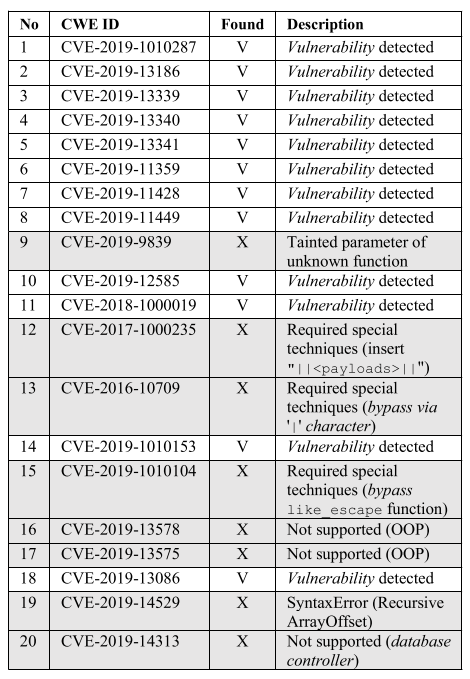
\includegraphics[scale=0.75]{static_experiment_table.PNG}
\caption{Testing Results \autocite[5]{Maskur2019}}
\end{figure}

\textcite[]{Maskur2019} mention a knowledge base which the tools needs to detect vulnerabilities. A better description of the knowledge base and the role of the security engineer that should improve the knowledge base would be helpful to assess the tool's potential. The test result only offer a superficial assessment of the static analysis tool and don't provide insights into the implementation.\newline  

In contrast \textcite[1170-1180]{Medeiros2019} provide a thorough description of the architecture and the implementation principles of SEPTIC. SEPTIC is tested with sets of 66 code examples taken, among other, from sqlmap \autocite[]{DameleA.G.2014} or other papers \autocite[]{Ray2012, Ray2014}. Furthermore the tool is tested against four other anti-SQL-Injection tools and a web application firewall. 61 of those samples were vulnerable code and five represented valid code. SEPTIC managed to detect all of the 61 attacks and did not deliver false positives. Due to the training mode and constructed query models SEPTIC was able to outperform the other tested security tools (see Figure \ref{septic1}).

\begin{figure*}
\centering
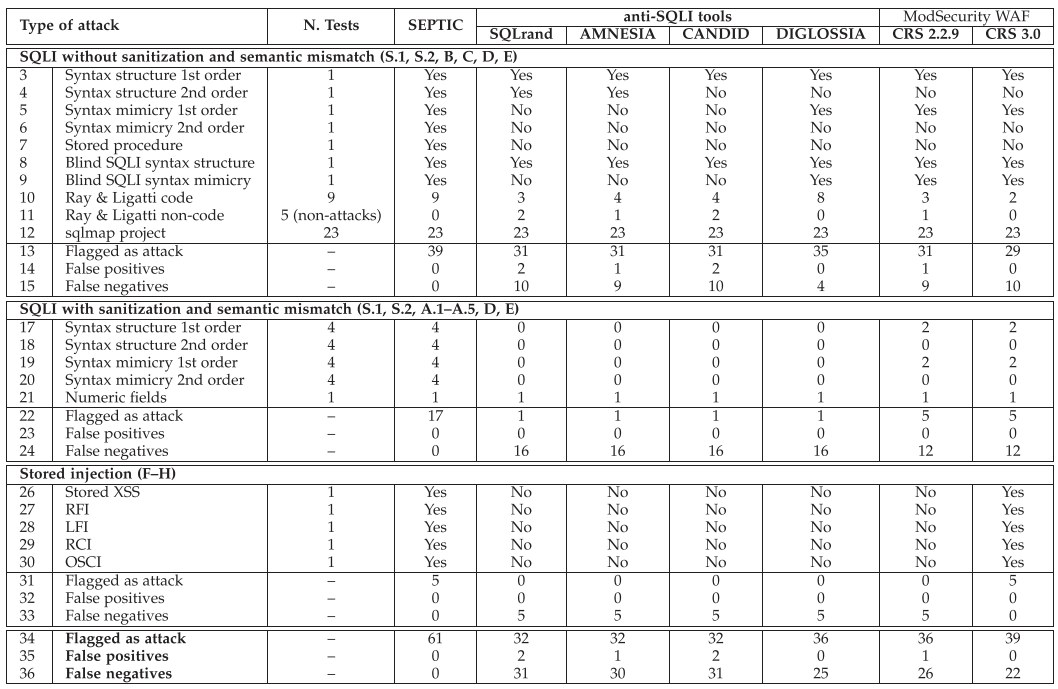
\includegraphics[scale=0.65]{septic_results.PNG}
\caption{SEPTIC:Code Sample Testing Results \autocite[1182]{Medeiros2019}}
\label{septic1}
\end{figure*}

SEPTIC performed well in a testing environment but the analysis tool was also tested with ten different open source PHP web application and one non-web application. Each application, apart from two, has known SQL or stored injection vulnerabilities. \textcite[]{Medeiros2019} used the wapiti scanner \autocite[]{Surribas2016} to perform attacks on the applications. SEPTIC was able to detect all attacks. The authors confirmed that there hadn't been any false positives or negatives by checking the logs containing all attacks performed.

\begin{figure}[H]
\centering
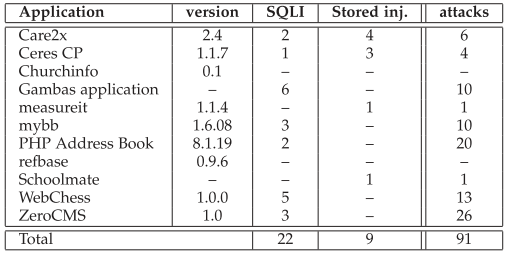
\includegraphics[scale=0.75]{septic_application_test.PNG}
\caption{SEPTIC: Application Testing Results \autocite[1183]{Medeiros2019}}
\end{figure}

By building the query models SEPTIC is able to correctly detect valid dynamic queries. The most distinct feature about SEPTIC is that it is located inside the DBMS. It is the first tool to be applied and perform directly in the database \autocite[1182f, 1186]{Medeiros2019}. Currently SEPTIC is focused on SQL injection. Further updates including more types of attacks would be an important feature for future development. It is an interesting approach to add another security layer directly at the database as it is easy to implement into an existing application as the tool doesn't need to know details about the whole source code.\newline


SQLBlock was evaluated through analysis of PHP web apps using Wordpress, Joomla, Drupal and Magento. Static analysis was performed on each application to identify the database access layer and then trained with each unit test included in each repository. Figure \ref{sqlblock} shows in column three each type of SQL-attack performed. SQLBlock blocked any of those SQL attack types whereas SEPTIC could only block against four and only in Wordpress plugins \autocite[11]{Jahanshahi2018}. The static analysis phase, training mode and the creating-profile phase are performed offline. Static analysis and creating the profile are automatically executed by SQLBlock without further help by the administrator. The administrator only executes the unit test for the training mode. False positives that were detected in especially Wordpress apps resulted from incomplete coverage during the training mode. Many dynamically generated queries rely on user input. Hence it is almost impossible to cover all benign queries in training mode \autocite[10-12]{Jahanshahi2018}. Due to the thorough analysis in the first three steps especially the analysis of the database access layer, SQLBlock can create query descriptors. Those descriptors contain many details of each query and therefore cover a lot of SQL attacks in contrast to SEPTIC that relies purely on the SQL-Syntax. Another important feature of SQLBlock is the ability to be used in popular CMS as a plugin.

\begin{figure*}
\centering
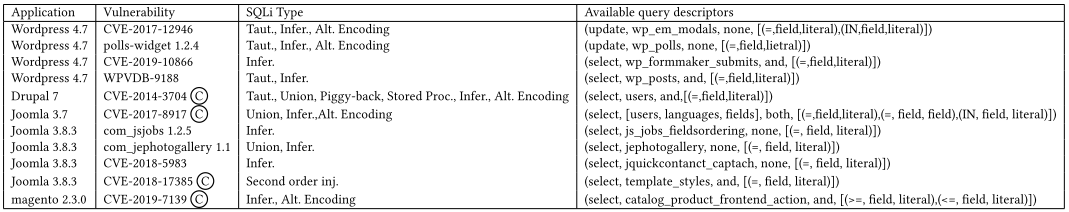
\includegraphics[scale=0.75]{sqlblock.PNG}
\caption{SQLBlock: Testing results \autocite[12]{Jahanshahi2018}}
\label{sqlblock}
\end{figure*}

\section{Summary}
Static analysis can only cover vulnerabilities in the source code and can improve the code quality. As many attack areas can only be detected in execution, dynamic analysis tools like SEPTIC could be more helpful. Hybrid tools like SQLBlock analyse apps more thoroughly and therefore can develop better defense mechanisms than other tools. The presented examples are mainly focused on the SQL injection vulnerability but there are many more tools to consider when implementing security features.





% h = try to place the figure Here
% t = try to place the figure at the Top of a page
% p = try to place this figure along with others on a separate Page
% Note that LaTeX has a sophisticated ranking algorithm to place figures.
% It is not always easy to accept LaTeX's placing but it is harder doing it
% manually. Just let it go ;-)

